\section{Experiment Results}

\subsection{Dataset and Preprocessing}

Among alternative available datasets~\cite{KDDCup, DARPA, UNSW1},
we choose NSL-KDD dataset~\cite{NSL-KDD} and UNSW-NB15 dataset~\cite{UNSW}
to evaluate the performance of various proposed neural networks in the network intrusion detection.

\subsubsection{NSL-KDD Dataset}
The NSL-KDD dataset originates from the KDDCup 99 dataset~\cite{KDDCup},
which was used for the third International Knowledge Discovery and Data Mining Tool Competition.
NSL-KDD dataset addresses two issues of the KDDCup 99 dataset.
First, it eliminates the redundant records existing in KDDCup 99, which takes up
78\% and 75\% of the records in train and test set, respectively.
Second, it samples the dataset such that the fraction of the record from a difficulty level
is inversely proportional to its difficulty.
Both enhancements make NSL-KDD dataset more suitable for
evaluating intrusion detection systems.

The train dataset consists of 125,973 TCP connection records, while the test dataset
consists of 22,544 ones.
A record is defined by 41 features, including 9 basic features of individual
TCP connections, 13 content features within a connection and 9 temporal features computed
within a two-second time window, and 10 other features.
Connections in the train dataset are labeled as either normal or one of the 24 attack
types.
There are additional 14 types of attacks in the test dataset, intentionally designed to
test the classifier's ability to handle novel attacks.
The task of the classifier is to identify whether a connection is normal or one of the
4 categories of attacks, namely denial of service (DoS), remote to local (R2L), user to
root (U2R) and probing, also known as 5-class classification problem.

\subsubsection{UNSW-NB15 Dataset}
Similar to KDDCup 99 dataset, the UNSW-NB15 dataset is generated by simulating normal
activities and attack behaviors in a testbed.
The simulation is conducted in the Cyber Range Lab of the Australian Centre for Cyber Security (ACCS)
and 49 features in the dataset is extracted by a chain of software tools also developed by ACCS.
The structure of the features is also similar to that of KDDCup 99: 5 flow features,
13 basic features, 8 content features, 9 time features and 12 other features.
The size of the dataset is 257,673 in term of flow records, 175,341 of which are used for
training set and the rest are for testing.
There are nine types of attacks in the dataset.
The only common type of attack between UNSW-NB15 and NSL-KDD is DoS.
The new attacks in UNSW-NB15 are analysis, backdoor, exploits, fuzzers, generic, reconnaissance, shellcode, and worms.
In this project, we consider the 2-class classification problem for UNSW-NB15 dataset: the
task of the classifiers is to predict a given traffic is either normal or malicious.

\subsubsection{Preprocessing}
Our data preprocessing starts with map the symbolic fields to a unique integer identifier.
For example, a data record from NSL-KDD dataset be one of the 5 types of traffic.
Therefore, its label will be mapped to 0, if normal, or to a number from 1 to 4 representing one of the four attacks.
A symbolic feature, like ``protocol" in both dataset, will be mapped to integer from 1 to $n$
where $n$ is the number of possible unique values.
We one-hot-encode only the label and features with small $n$.
That is, a feature or a label of value $x$ will be converted to a $n$-dimensional binary vector
with the $x$th dimension set to 1 and others set to zero.
Then we shuffled the data, together with its labels, so that later in the stochastic
gradient descent learning phase, batch data are already randomized.
At last, we perform the min-max normalization so that data values are all in the range
of [0, 1].


\subsection{Evaluation Metrics}
We evaluate the classification performance of our proposed deep learning approaches
with the following metrics.
\begin{itemize}
    \item \textbf{Accuracy} is the percentage of correctly classified connections
        over the total number of connections in the dataset:
        \begin{align}
            A = \frac{\text{Correct Predictions}}{\text{Number of Records}}
        \end{align} 
        Accuracy is not suitable for evaluating biased dataset where the number
        of records of some class is extremely larger than the number of
        records of another class.
        In NSL-KDD dataset, the number of available U2R records (67)
        is in two degrees of magnitude less than the other classes of traffic
        (9711, 7458, 2887, 2121 respectively).
        Therefore we also consider the following metrics.
    \item \textbf{Precision} is the percentage of the correctly classified positives over
        the total number of positives predicted by the classifier:
                \begin{align}
                    P = \frac{\text{True Positives}}{\text{True Positives} + \text{False Positives}}
                \end{align}
    \item \textbf{Recall} is the percentage of the correctly classified positives over
        the total number of relevant elements:
                \begin{align}
                    R = \frac{\text{True Positives}}{\text{True Positives} + \text{False Negatives}}
                \end{align}
    \item \textbf{F1-Score} represents a balance between precision and recall and is calculated
        as their harmonic mean:
                \begin{align}
                    F = \frac{2PR}{P + R}
                \end{align}
\end{itemize}
In the 5-class classification, we calculate the precision, recall and F1-Score for each traffic class.
Additionally, we report the weighted average of these metrics as a single value for comparing various approaches.
The weight for each class is determined by its proportion in the test dataset.
The weight vector for class [Normal, Probe, DoS, U2R, R2L] is [0.431, 0.107, 0.339, 0.018, 0.105].
Besides, we also provide the confusion matrix of the classification results when applying
different approaches on the test dataset.
In our confusion matrix table, the row represents the instance in an actual class,
while the column represents the instance in a predicted class.
It is called confusion matrix because it is useful for visualizing how a classifier
is confusing one class with other classes.


\subsection{Performance of Deep Learning Approaches}
First we report the classification accuracy of each considered approach
applied on NSL-KDD dataset in Figure~\ref{Fig:CompAccuracy}.

Surprisingly, the most ``accurate" approach is the simple 16-neuron perceptron (81.42\%).
Sparse autoencoder based self-taught leaner achieved second best accuracy of 79.15\%.
This number coincides with the previously reported results in~\cite{STL-NIDS} (79.10\%).
RBM and denoising autoencoder have similar accuracy results (77.58\% and 76.93\%).

\begin{figure}[h]
    \centering
    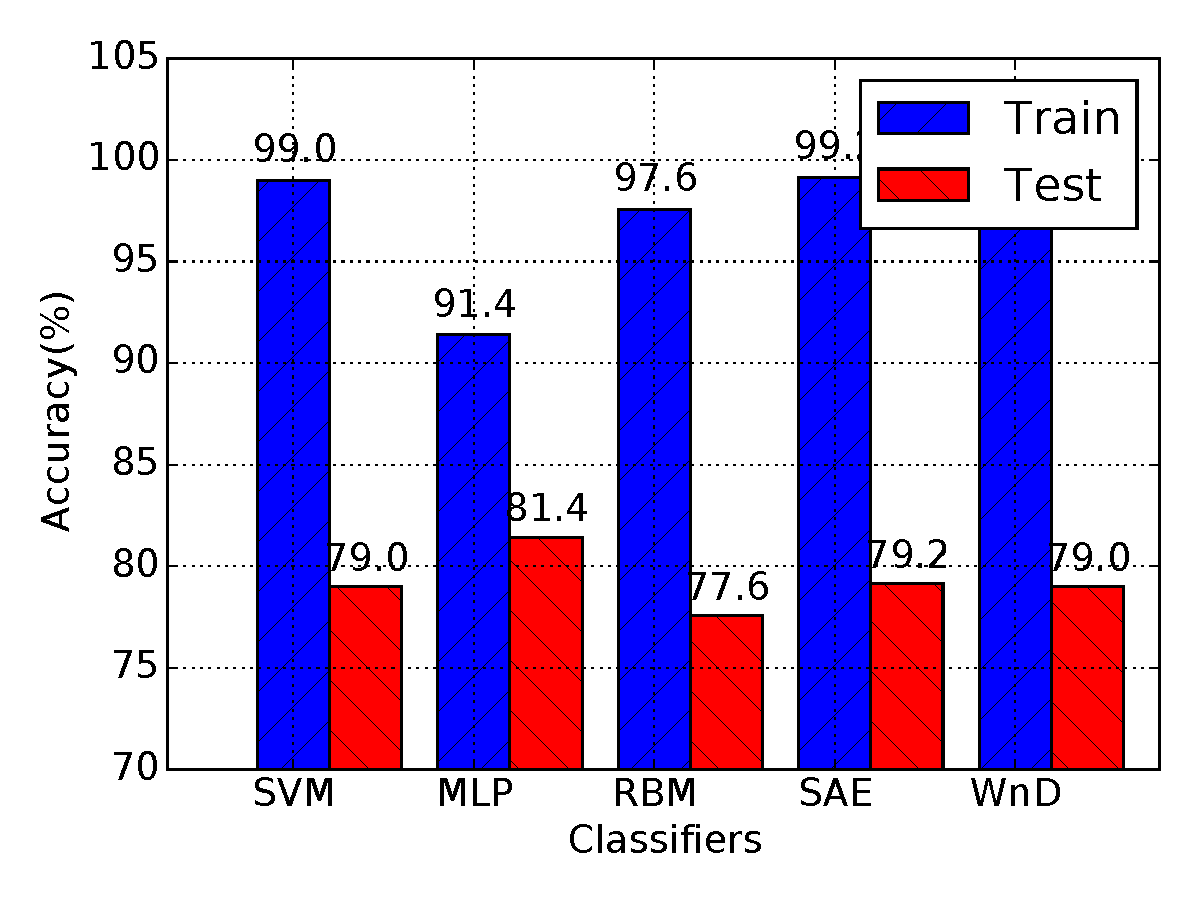
\includegraphics[width=0.48\textwidth]{figures/comp_accuracy.pdf}
    \caption{Classification Accuracy of Proposed Approaches on NSL-KDD Dataset}
    \label{Fig:CompAccuracy}
\end{figure}

Table~\ref{Tab:ConfusionMatrixMLP} --~\ref{Tab:ConfusionMatrixDAE} summarize the confusion matrices
of each approach and their weighted average metrics (Precision, Recall and F1-Score).
Apart from best accuracy, MLP also achieved the best F1-Score (80.44\%)
among all of the considered approaches.
However, we can see that for U2R attacks, MLP still has very poor results of
both precision (13.95\%) and recall (10.35\%).
The second highest F1-Score is achieved by sparse autoencoder combined with softmax regression (78.05\%).
This value is actually a little bit higher than the result (75.76\%) reported in~\cite{STL-NIDS}.
We believe this is partly due to the reason that we did not introduce regularization
for both sparse autoencoder and softmax regression classifier,
and partly due to the dropout technique we used in training the softmax regression classifier.
RBM and DAE again achieve very similar classification performance,
with F1-Score of 75.63\% and 75.65\% respectively.
Considering both the high accuracy and best F1-Score, we conclude that in the competition of
5-class classification, MLP is the winner.

Confusion matrices here tell us something interesting about the classification performance
for each type of traffics.
MLP correctly recognized the most number of normal traffics (9329 out of 9711).
For the attacking traffics, the winner classifier MLP correctly predicted the most
number of DoS attacks (6146 out of 7636), U2R attacks (41 out of 396)
and R2L attacks (926 out of 2376).
RBM is the best classifier in predicting Probe attacks (2015 out of 2425).

The wide and deep learning model, as stated in Section~\ref{SubSec:WD},
(WnD) requires us engineering the features of UNSW dataset into
basis, crossed, continuous, indicator and embedded components.
The basis features are all the raw symbolic and integer features.
These basis features are also fed to the deep model after conducting the embedding step.
The continuous features are all the raw continuous features.
We make the full combinations of symbolic features to be crossed features.
For comparison reason, we set the structure of the deep neural network in WnD to be
the same sizes as that of the baseline neural network,
namely three hidden layers with sizes of [480, 512, 640].
As the result shows, augmenting the deep neural network with wide linear regressor
provides a 3\% increase in accuracy to the baseline three-layer neural network.

\begin{figure}[h]
    \centering
    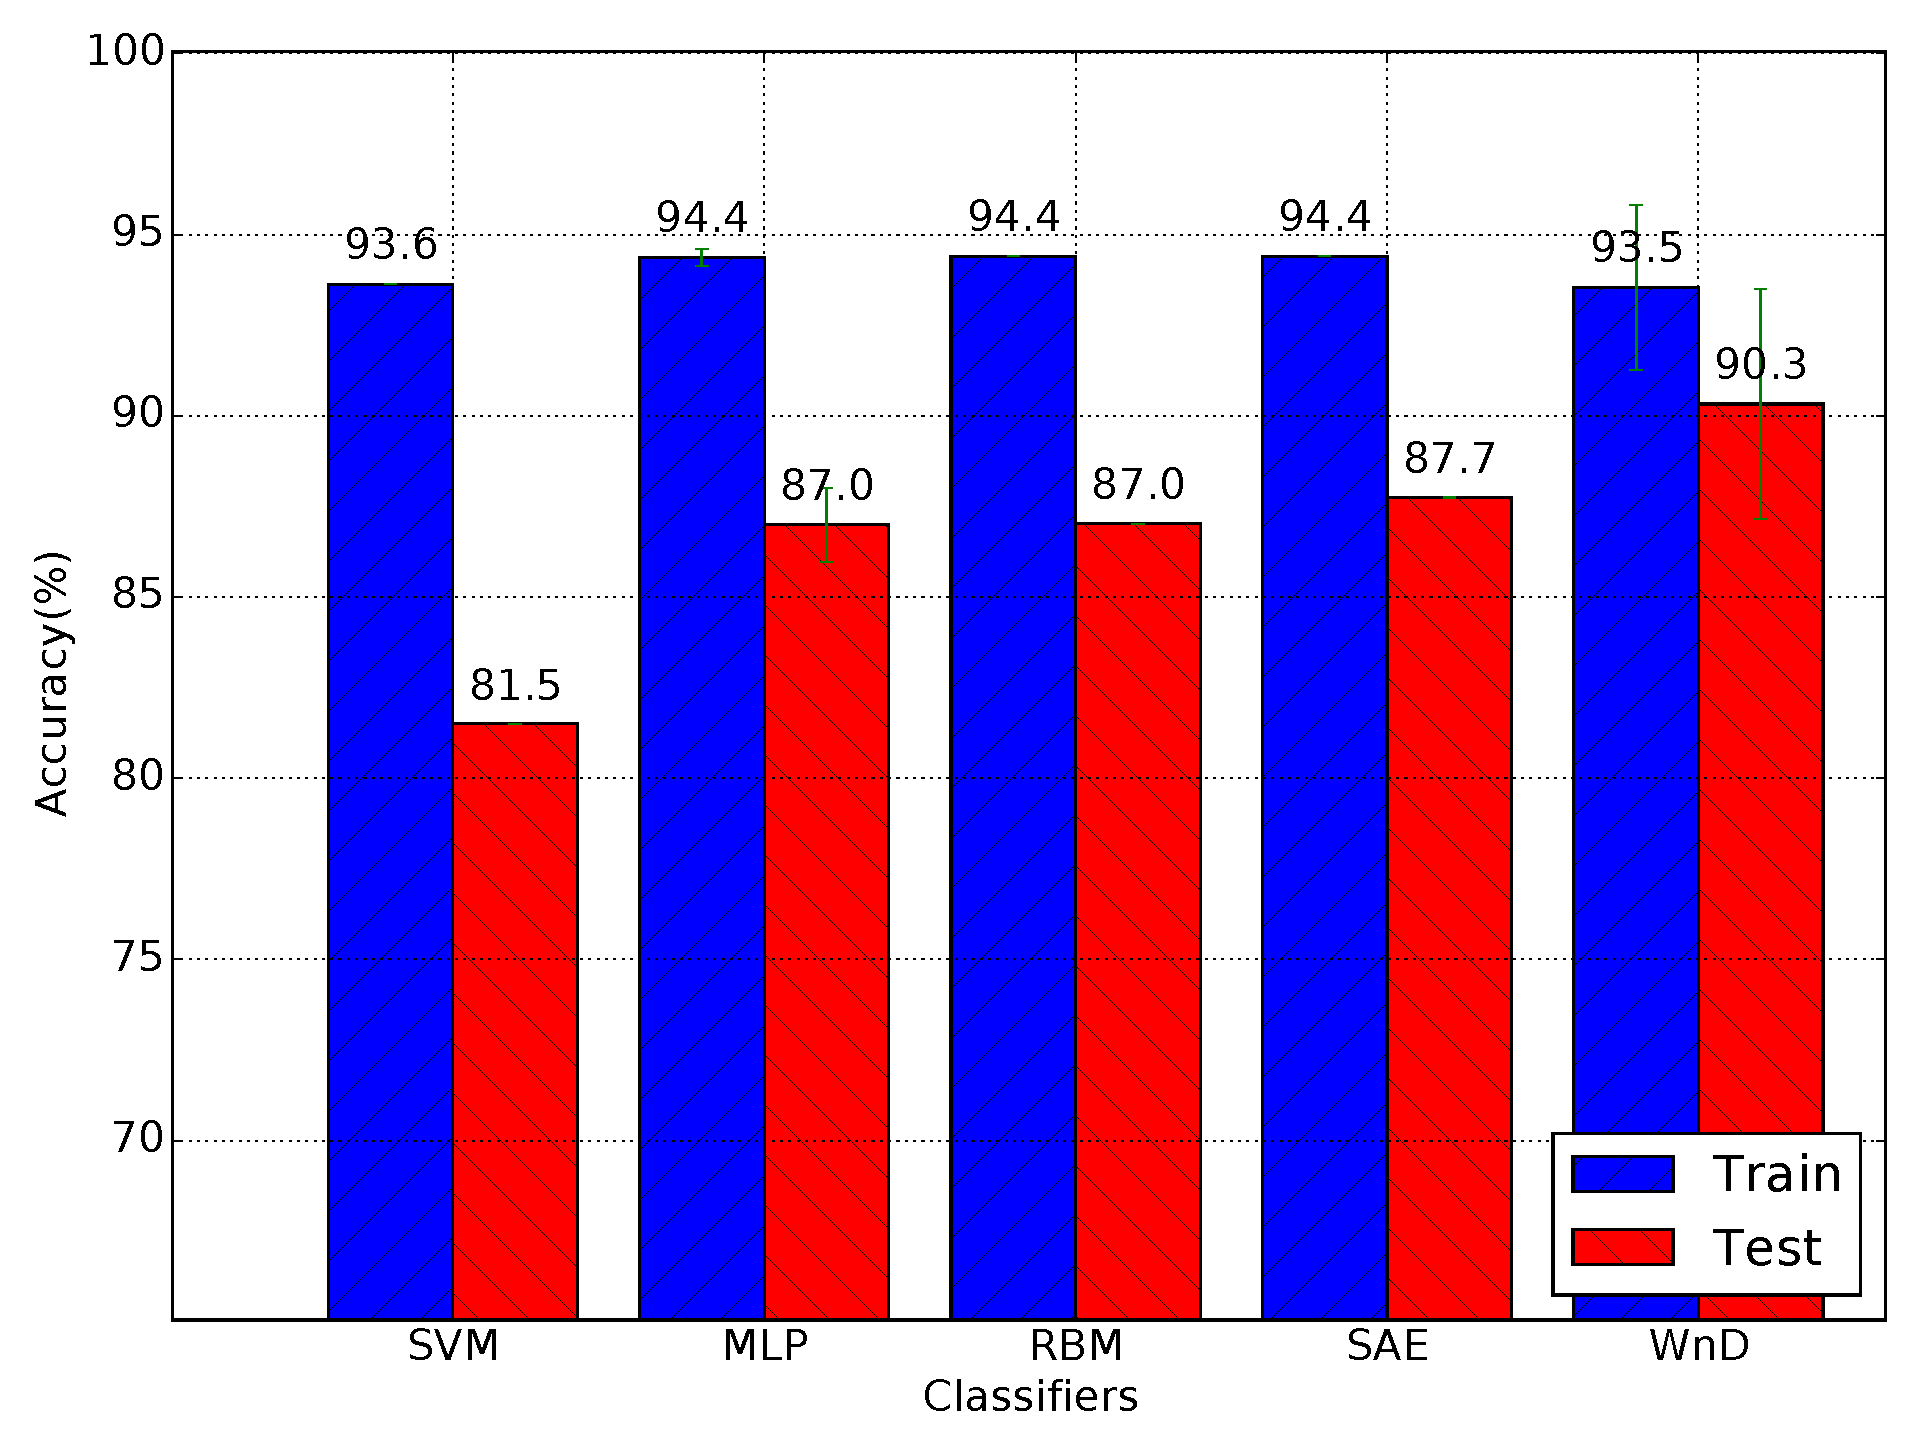
\includegraphics[width=0.48\textwidth]{figures/comp_accuracy_unsw.pdf}
    \caption{Classification Accuracy of Proposed Approaches on UNSW-NB15 Dataset}
    \label{Fig:CompAccuracyUNSW}
\end{figure}

\iffalse
\begin{table}[t]
    \caption{Confusion Matrix of MLP on Test Dataset}
    \centering
    \begin{tabular}{cc|rrrrr}
        \hline
        &  & \multicolumn{5}{c}{Prediction} \\
                        &        & Normal & Probe & DoS & U2R & R2L\\
        \hline
        \hline
        \multirow{5}{*}{Actual} & Normal & {\color{red}9329} &  230 &   70 &  25 &  57 \\
                                &  Probe &  164 & 1914 &  271 &  10 &  66 \\
                                &  DoS   & 1358 &   82 & {\color{red}6146} &  47 &   3 \\
                                &  U2R   &  345 &    4 &    0 &  {\color{red}41} &   6 \\
                                &  R2L   & 1247 &   30 &    2 & 171 & {\color{red}926} \\
        \hline
        \multicolumn{2}{c|}{Precision(\%)}   & 74.97 & 84.69 & 94.71 & 13.95 & 87.52\\
        \multicolumn{2}{c|}{Wtd. Avg.(\%)}   & \multicolumn{5}{r}{82.96}\\
        \hline
        \multicolumn{2}{c|}{Recall(\%)}      & 96.07 & 78.93 & 80.49 & 10.35 & 38.97\\
        \multicolumn{2}{c|}{Wtd. Avg.(\%)}   & \multicolumn{5}{r}{81.42}\\
        \hline
        \multicolumn{2}{c|}{F1-Score(\%)}    & 84.22 & 81.71 & 87.02 & 11.88 & 53.93\\
        \multicolumn{2}{c|}{Wtd. Avg.(\%)}   & \multicolumn{5}{r}{\textbf{\color{red}80.44}}\\
        \hline
    \end{tabular}
    \label{Tab:ConfusionMatrixMLP}
\end{table}


\begin{table}[t]
    \caption{Confusion Matrix of RBM on Test Dataset}
    \centering
    \begin{tabular}{cc|rrrrr}
        \hline
        &  & \multicolumn{5}{c}{Prediction} \\
                        &        & Normal & Probe & DoS & U2R & R2L\\
        \hline
        \hline
        \multirow{5}{*}{Actual} & Normal & 8903 &  318 &  428 &  11 &   51 \\
                                & Probe  &  232 & {\color{red}2015} &  159 &   2 &   17 \\
                                & DoS    & 1879 &  143 & 5613 &   0 &    1 \\
                                & U2R    &  356 &    3 &    1 &  27 &    9 \\
                                & R2L    & 1550 &    8 &    1 &   8 &  809 \\
        \hline
        \multicolumn{2}{c|}{Precision(\%)}   & 68.91& 81.02& 90.50& 56.25& 91.21\\
        \multicolumn{2}{c|}{Wtd. Avg.(\%)}   & \multicolumn{5}{r}{79.65}\\
        \hline
        \multicolumn{2}{c|}{Recall(\%)}      & 91.68& 83.09& 73.51&  6.82& 34.05\\
        \multicolumn{2}{c|}{Wtd. Avg.(\%)}   & \multicolumn{5}{r}{77.04}\\
        \hline
        \multicolumn{2}{c|}{F1-Score(\%)}    & 78.68& 82.04& 81.12& 12.16& 49.59\\
        \multicolumn{2}{c|}{Wtd. Avg.(\%)}   & \multicolumn{5}{r}{75.63}\\
        \hline
    \end{tabular}
    \label{Tab:ConfusionMatrixRBM}
\end{table}

\begin{table}[t]
    \caption{Confusion Matrix of SAE on Test Dataset}
    \centering
    \begin{tabular}{cc|rrrrr}
        \hline
        &  & \multicolumn{5}{c}{Prediction} \\
                        &        & Normal & Probe & DoS & U2R  & R2L\\
        \hline
        \hline
        \multirow{5}{*}{Actual}  & Normal & 8864 &  696 &   92 &   11 &   48 \\
                                 & Probe  &  179 & 2001 &  164 &    2 &   79 \\
                                 & DoS    & 1542 &   39 & 6054 &    0 &    1 \\
                                 & U2R    &  357 &    1 &    1 &   30 &    7 \\
                                 & R2L    & 1444 &    6 &    5 &   26 &  895 \\
        \hline
        \multicolumn{2}{c|}{Precision(\%)}    & 71.56& 72.95& 95.85& 43.48& 86.89\\
        \multicolumn{2}{c|}{Wtd. Avg.(\%)}    & \multicolumn{5}{r}{81.06}\\
        \hline
        \multicolumn{2}{c|}{Recall(\%)}       & 91.28& 82.52& 79.28&  7.58& 37.67\\
        \multicolumn{2}{c|}{Wtd. Avg.(\%)}    & \multicolumn{5}{r}{79.15}\\
        \hline
        \multicolumn{2}{c|}{F1-Score(\%)}     & 80.23& 77.44& 86.78& 12.90& 52.55\\
        \multicolumn{2}{c|}{Wtd. Avg.(\%)}    & \multicolumn{5}{r}{78.05}\\
        \hline
    \end{tabular}
    \label{Tab:ConfusionMatrixSAE}
\end{table}


\begin{table}[t]
    \caption{Confusion Matrix of DAE on Test Dataset}
    \centering
    \begin{tabular}{cc|rrrrr}
        \hline
        &  & \multicolumn{5}{c}{Prediction} \\
                        &        & Normal & Probe & DoS & U2R & R2L\\
        \hline
        \hline
        \multirow{5}{*}{Actual} & Normal & 9249 &  319 &   85 &  10 &  48 \\
                                & Probe  & 576  & 1504 &  226 &   2 & 117 \\
                                & DoS    & 1842 &  128 & 5665 &   0 &   1 \\
                                & U2R    & 353  &    1 &    0 &  38 &   4 \\
                                & R2L    & 1469 &    3 &    1 &  17 & 886 \\
        \hline
        \multicolumn{2}{c|}{Precision(\%)} & 68.57& 76.93& 94.78& 56.72& 83.90\\
        \multicolumn{2}{c|}{Wtd. Avg.(\%)} & \multicolumn{5}{r}{79.75}\\
        \hline
        \multicolumn{2}{c|}{Recall(\%)}    & 95.24& 62.02& 74.19&  9.60& 37.29\\
        \multicolumn{2}{c|}{Wtd. Avg.(\%)} & \multicolumn{5}{r}{76.93}\\
        \hline
        \multicolumn{2}{c|}{F1-Score(\%)}  & 79.73& 68.68& 83.23& 16.41& 51.63\\
        \multicolumn{2}{c|}{Wtd. Avg.(\%)} & \multicolumn{5}{r}{75.65}\\
        \hline
    \end{tabular}
    \label{Tab:ConfusionMatrixDAE}
\end{table}
\fi
